\lstdefinelanguage{VS}{
    alsoletter={<, >, /, \#, _},
    keywords=[1]{\#define, \#include},
    keywordstyle=[1]\color{gray},
    keywords=[2]{<experimental/filesystem>},
    keywordstyle=[2]\color{lorange},
    keywords=[3]{_SILENCE_EXPERIMENTAL_FILESYSTEM_DEPRECATION_WARNING},
    keywordstyle=[3]\color{purple},
    sensitive=false, % keywords are not case-sensitive
    morecomment=[l]{}, % l is for line comment
    morecomment=[s]{/*}{*/}, % s is for start and end delimiter
    morestring=[b]" % strings are enclosed in double quotes
}%
\lstset{language=VS}

\section{Build Instructions}
\label{sec:buildinstructions}

\subsection{WinDbg Crash Analyse}
\label{subsec:build_windbg}

Benötigte Tools:
\begin{itemize}
    \item Windows Betriebssystem
    \item WinDbg Preview \cite{misc:windbgpreview}
    \item Crash Dumb des Bugs\footnotemark
    \item Symbol-Dateien des Codes -> GEOPAK64.pdb, MnGeom364.pdbS \footnotemark[\value{footnote}] \footnotetext{Erreichbar unter H:\textbackslash thomasW\textbackslash v\_DB}
    \item Zugriff auf Azure DevOps Server von Mitutoyo-CTL Germany GmbH
\end{itemize}

Um den Crash Dump nun zu analysieren, wird dieser mit WinDbg Preview über die Funktion \glqq{}Open dump file\grqq{} geöffnet.
Die darauf folgenden Schritte sind bereits in \ref{sec:windbg} beschrieben.


\subsection{Kompilieren von Mitutoyo.MCOSMOS.BasicLibs}
\label{subsec:build_code}

Benötigte Tools:
\begin{itemize}
    \item Windows Betriebssystem
    \item Visual Studio 2017 oder Visual Studio 2019 ohne Updates
    \item Zugriff auf den Azure DevOps Serever von Mitutoyo-CTL Germansy GmbH
    \item Git Extensions oder ein ähnliches Tool zum Klonen von Git Repositorys
\end{itemize}

Damit der Source Code kompiliert werden kann, muss dieser zuest mit Git Extensions (oder einem ähnlichen Tool) von
\url{http://tfs-ctlg.mitutoyo-ctl.de/Public/Projects/_git/Mitutoyo.MCOSMOS.BasicsLibs} geklont werden. Damit der Bug noch vorhanden ist, sollte der Source Code vom Stand des
Commits \verb|bb882af1| verwendet werden. \newline
Anschließend öffnet man die Projekt-Datei \textit{Mitutoyo.MCOSMOS.BasicsLibs\textbackslash Source\textbackslash MBa\allowbreak sicsLibs.sln} mit Visual Studio.

\begin{figure}[htpb]
    \centering
    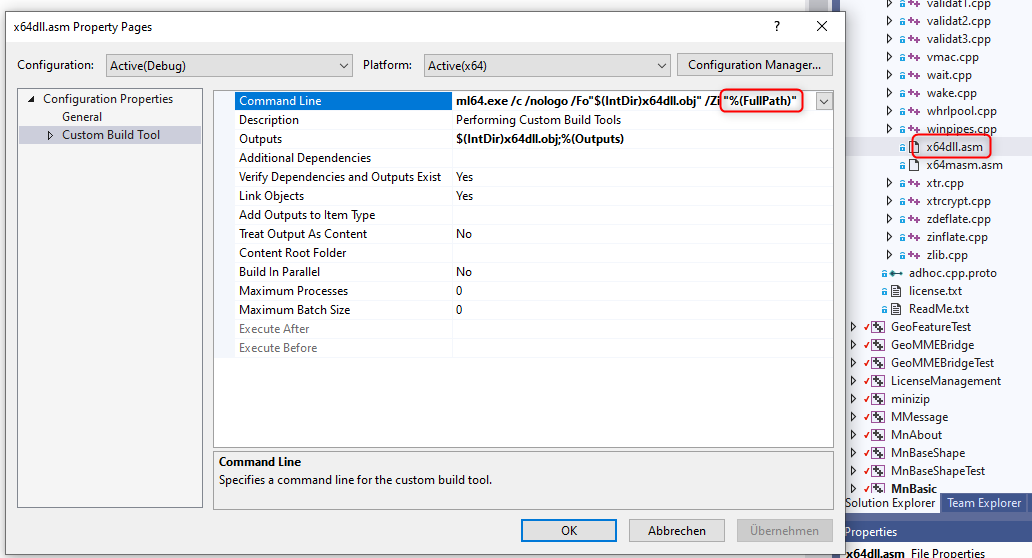
\includegraphics[width=0.85\textwidth]{x64dll_correction}
    \caption{Durchzuführende Korrektur}
    \label{img:x64dll_correction}
\end{figure}

Da \gls{masm} keine Leerzeichen im Pfadname verarbeiten kann, muss in den Eigenschaften der Datei
\textit{Mitutoyo.MCOSMOS.BasicsLibs\textbackslash Source\textbackslash CryptoPP\textbackslash x64dll.asm} unter \glqq{}Custom Build Tool\grqq{}
-> \glqq{}General\grqq{} -> \glqq{}Command Line\grqq{} folgender Eintrag eingegeben werden: \textit{ml64.exe /c /nologo /Fo"\$(IntDir)x64dll.obj" /Zi "\%(FullPath)"}
(vgl. \ref{img:x64dll_correction}).

Des Weiteren muss in der Datei \textit{IniFileHelper.h} folgender Code ergänzt werden:
\begin{lstlisting}
14    #define _SILENCE_EXPERIMENTAL_FILESYSTEM_DEPRECATION_WARNING
15    #include <experimental/filesystem>
\end{lstlisting}

Zuletzt muss die Operation \glqq{}Restore NuGet Packages\grqq{}, über einen Rechtsklick auf die Solution, ausgewählt und ausgeführt werden.

Der Code kann nun kompiliert werden.